% Phase 2 results. Every number resolves through a macro in numbers.tex,
% written by make_report_numbers.py from the run records.

\begin{table*}[t]
\centering\small
\begin{tabular}{lrrrrrr}
\toprule
\textbf{arm} & \textbf{seeds} & \textbf{final val ppl} & \textbf{steps to 45} & \textbf{sec to 45} & \textbf{train s} & \textbf{peak GiB} \\
\midrule
baseline & 6 & 40.54 {\scriptsize$\pm$ 0.33} & 2,915 {\scriptsize$\pm$ 48} & 381 & 523 & 7.40 \\
attn-first & 6 & 41.63 {\scriptsize$\pm$ 0.81} & 3,096 {\scriptsize$\pm$ 165} & 405 & 523 & 7.40 \\
attn-second & 6 & 40.16 {\scriptsize$\pm$ 0.15} & 2,774 {\scriptsize$\pm$ 23} & 363 & 524 & 7.40 \\
attn-first-lrm & 6 & 41.07 {\scriptsize$\pm$ 0.60} & 2,993 {\scriptsize$\pm$ 103} & 389 & 520 & 7.40 \\
attn-second-lrm & 6 & 40.21 {\scriptsize$\pm$ 0.17} & 2,788 {\scriptsize$\pm$ 22} & 365 & 523 & 7.40 \\
alternating & 3 & 40.65 {\scriptsize$\pm$ 0.56} & 2,914 {\scriptsize$\pm$ 85} & 385 & 530 & 7.40 \\
attn-freeze & 3 & 53.91 {\scriptsize$\pm$ 0.56} & --- & --- & 512 & 7.40 \\
\bottomrule
\end{tabular}
\caption{Phase~2 results, mean $\pm$ SD over seeds. ``steps to 45'' and ``sec to 45'' are the training step and training seconds at which validation perplexity first reaches 45 (interpolated; --- if never reached). ``train s'' is total training time and ``peak GiB'' the peak GPU memory. At a given seed every arm shares the baseline's initialization and data order.}
\label{tab:p2}
\end{table*}


\begin{figure}[t]
\centering
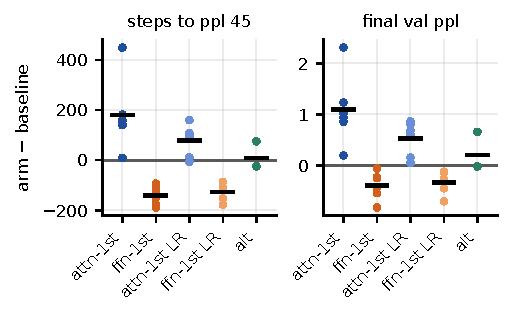
\includegraphics[width=\columnwidth]{figures/figp_paired.pdf}
\caption{Per-seed differences from the baseline (each point is one seed; the
bar is the mean). 
Left shows difference in step count to reach perplexity 45. 
Right shows difference in final perplexity value.
Below zero means the arm beat the baseline for that seed.
``LR'' marks the learning-rate-matched arms. attn-freeze (+13 perplexity) is
left out for scale.}
\label{fig:paired}
\end{figure}

Table~\ref{tab:p2} lists every arm, and Figure~\ref{fig:paired} shows the
per-seed differences from the baseline.

% \paragraph{FFN first helps.} attn-second beats the baseline in all
% \ASStepsNseeds{} seeds: \ASStepsDiffAbsInt{} fewer steps to perplexity
% \TargetPpl{} ($-\ASStepsRelAbs$\%, $p \ASStepsP$) and $-\ASPplRelAbs$\% final
% perplexity ($p \ASPplP$). This arm also gives the FFN \BudgetEarlyPct\% more
% total learning rate than the baseline, so the gain could come from the larger
% budget alone. attn-second-lrm removes that difference and keeps most of the
% gain: $-\ASLStepsRelAbs$\% steps and $-\ASLPplRelAbs$\% final perplexity, again
% better than the baseline in every seed ($p \ASLStepsP$ for both). The
% advantage of emphasising the FFN early is therefore not a budget effect.

% \paragraph{Attention first hurts.} attn-first is worse than the baseline in
% every seed ($+\AFStepsRelAbs$\% steps, $+\AFPplRelAbs$\% final perplexity,
% $p \AFStepsP$ for both). With the budget matched, attn-first-lrm is still
% worse, by about half as much: $+\AFLStepsRelAbs$\% steps (worse in
% \AFLStepsWorse{} of \AFLStepsNseeds{} seeds, $p \AFLStepsP$) and
% $+\AFLPplRelAbs$\% final perplexity (\AFLPplWorse{} of \AFLPplNseeds{},
% $p \AFLPplP$). So about half of the original penalty came from the budget.
% Compared directly, the two matched arms separate in \AFLvASLStepsWorse{} of
% \AFLvASLStepsNseeds{} seeds on both metrics ($p \AFLvASLStepsP$).

% These $p$-values are the smallest possible with six seeds, so they mean
% ``every seed agreed'' rather than a precise probability. The effects are
% small: a few percent in steps, about 1\% in final perplexity.

\paragraph{Training the FFN first helps.} Emphasising the FFN before the
switch step makes training faster in every seed: attn-second needs
\ASStepsRelAbs\% fewer steps to reach perplexity \TargetPpl{} and ends with
slightly lower perplexity. This arm also gives the FFN more total learning
rate than the baseline (Section~\ref{sec:arms}), so the gain could have come
from the extra learning rate alone. To check this, attn-second-lrm uses
the same timing with the total learning rate matched to the baseline. It
keeps almost all of the gain (\ASLStepsRelAbs\% fewer steps), again in every
seed. What helps is therefore \emph{when} the FFN is emphasised, not how much
learning rate it gets.

\paragraph{Training attention first hurts.} The mirror image, attn-first, is
slower than the baseline in every seed. About half of this penalty came from
the learning-rate imbalance: with the total matched, attn-first-lrm is still
worse, but by roughly half as much, and no longer in every seed. Compared
directly, the two matched arms still differ in every seed, so the order in
which the two groups are emphasised matters.

\paragraph{How large are these effects?} Small. The best arm saves about
\ASLStepsRelAbs\% of the training steps and improves the final perplexity by
under 1\%. Every seed agrees on the direction, so the effects are consistent,
but they are about how fast the model trains, not how good it becomes.

\paragraph{Alternating has no effect.} alternating is indistinguishable from
the baseline ($\AltPplDiff$ perplexity, $p \AltPplP$; $\AltStepsDiffInt$ steps,
$p \AltStepsP$; \AltSeeds{} seeds) and its curve lies on the baseline's
(Figure~\ref{fig:curves}). Changing the emphasis without the Phase~1 timing
does not help.

\begin{figure}[t]
\centering
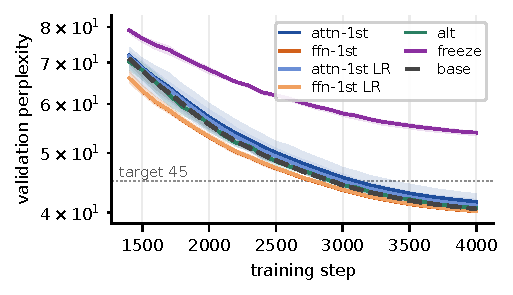
\includegraphics[width=\columnwidth]{figures/figp_curves.pdf}
\caption{Validation perplexity over the last two thirds of training (line:
mean over seeds; band: min--max). The baseline is dashed; alternating lies on
it. Both FFN-first arms (orange) stay below it.}
\label{fig:curves}
\end{figure}

\paragraph{Freezing hurts and saves little.} attn-freeze sets attention's
learning rate to zero after each layer's switch point, which falls 8--21\% of
the way into training. Attention's total weight displacement drops to
\FrzDispAttn{}, against \BaseDispAttn{} in the baseline, so attention really
stops learning. Final perplexity is \FrzPpl{} (\FrzPplRelAbs\% worse), and the
target of \TargetPpl{} is never reached. Training time drops by
\FrzWallRelAbs\% (\FrzWallDiffAbs{}\,s of \BaseWall{}\,s, 3 seeds).

% \paragraph{Manipulation check.} The weight displacement moves as designed
% (Figure~\ref{fig:disp}): attn-first moves attention more than the baseline
% (\AFDispAttn{} vs \BaseDispAttn) and the FFN less (\AFDispFfn{} vs
% \BaseDispFfn); attn-second does the reverse (\ASDispAttn{}, \ASDispFfn).
